\section{The Advantage Of Traces}
\label{sec:nanomaly:advantage-traces}
Finally, having shown that \toolname produces small traces in an
efficient manner, let us discuss the explanatory power of traces
compared with typical type error messages. In this section we will
present a qualitative evaluation of \toolname's jump-compressed traces
on a series of examples drawn from real student programs in the
\ucsdbench dataset. For each example we will present the code, a
jump-compressed trace produced by \toolname, and the type error produced
by the \ocaml compiler.

\begin{figure*}[ht]
\centering
\begin{minipage}{0.49\linewidth}
\centering
\begin{ecode}
let rec sqsum xs = match xs with
  | [] -> 0
  | h::t -> __(sqsum t)__ @ (h * h)
\end{ecode}
% File "sqsum.ml", line 3, characters 12-21:
\begin{verbatim}
Error: This expression has type
         int
       but an expression was expected of type
         'a list
\end{verbatim}
\end{minipage}
\begin{minipage}{0.49\linewidth}
\centering
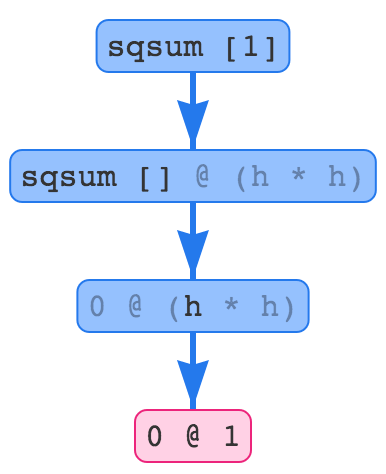
\includegraphics[height=125px]{sqsum.png}
\end{minipage}
\caption{\texttt{sqsum xs} should square each element of \texttt{xs} and
  then compute the sum of the result, but the student has used the
  list-append operator |@| instead of \texttt{+} to compute the
  sum. \ocaml blames the recursive call \texttt{sqsum t} (underlined
  above) for being an \texttt{int} instead of a \texttt{list}.
  \toolname's jump-compressed trace draws the eye to the
  entire term \texttt{0 }|@|\texttt{ 1}.}
\label{fig:trace-sqsum}
\end{figure*}

\begin{figure*}[ht]
\centering
\begin{minipage}{0.49\linewidth}
\centering
\begin{ecode}
let rec sumList xs = match xs with
  | []    -> []
  | y::ys -> y + __sumList ys__
\end{ecode}
% File "sumList.ml", line 3, characters 17-27:
\begin{verbatim}
Error: This expression has type
         'a list
       but an expression was expected of type
         int
\end{verbatim}
\end{minipage}
\begin{minipage}{0.49\linewidth}
\centering
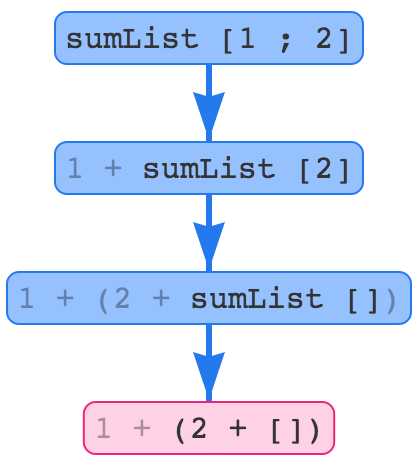
\includegraphics[height=125px]{sumlist.png}
\end{minipage}
\caption{\texttt{sumList xs} should sum the elements of \texttt{xs}, but
  the student has returned \texttt{[]} in the base case instead of
  \texttt{0}. \ocaml deduces from the base case that \texttt{sumList}
  must return a \texttt{list} and thus blames the recursive call on line
  3 for producing a \texttt{list} instead of an  \texttt{int}.
  \toolname's jump-compressed trace highlights the clash
  between the \texttt{[]} and the \texttt{+}, but also demonstrates in
  the third step that \texttt{sumList []} reduces to \texttt{[]}, which
  clarifies that the conflict is between the base case and recursive
  case.}
\label{fig:trace-sumlist}
\end{figure*}

\begin{figure*}[ht]
\centering
\begin{minipage}{0.49\linewidth}
\centering
\begin{ecode}
let append xs ys = match xs with
  | []   -> ys
  | h::t -> h :: __t__ :: ys
\end{ecode}
% File "append.ml", line 3, characters 17-18:
\begin{verbatim}
Error: This expression has type
         'a list
       but an expression was expected of type
         'a
       The type variable 'a occurs inside 'a list
\end{verbatim}
\end{minipage}
\begin{minipage}{0.49\linewidth}
\centering
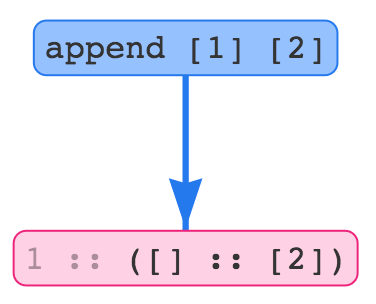
\includegraphics[height=75px]{append.png}
\end{minipage}
\caption{\texttt{append xs ys} should concatenate the two input lists,
  but the student has tried to cons the tail of \texttt{xs} onto
  \texttt{ys} instead of making a recursive call to \texttt{append}.
  \ocaml blames \texttt{t} on line 3 for being a \texttt{'a list}
  instead of a \texttt{'a}, prompting an \emph{occurs-check}
  error. \toolname shows, more concretely, that \texttt{[] :: [2]} gets
  stuck because lists are homogeneous and \texttt{[]} is not an
  \texttt{int}.}
\label{fig:trace-append}
\end{figure*}

\begin{figure*}[ht]
\centering
\begin{minipage}{0.49\linewidth}
\centering
\begin{ecode}
let rec wwhile (f,b) =
  match f with
  | (z, false) -> z
  | (z, true)  -> wwhile (f, z)

let f x =
  let xx = x * x in
  (xx, (xx < 100))

let _ = wwhile (__f__, 2)
\end{ecode}
% File "wwhile.ml", line 10, characters 16-17:
\begin{verbatim}
Error: This expression has type
         int -> int * bool
       but an expression was expected of type
         'a * bool
\end{verbatim}
\end{minipage}
\begin{minipage}{0.49\linewidth}
\centering
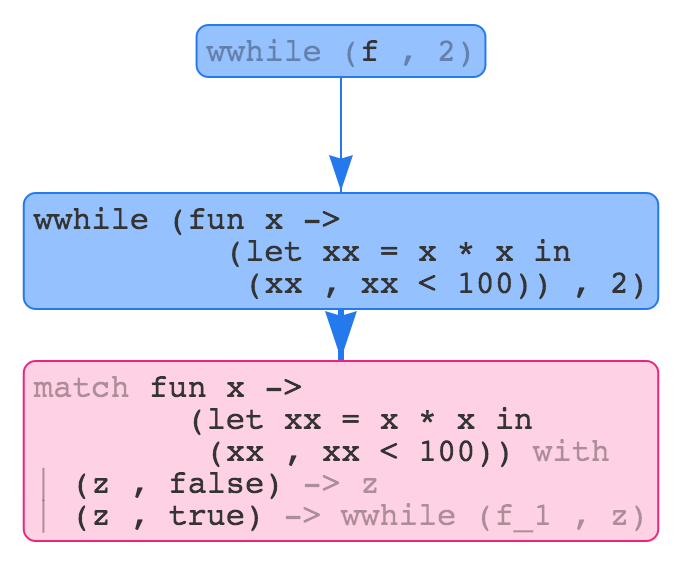
\includegraphics[height=150px]{wwhile.png}
\end{minipage}
\caption{\texttt{wwhile (f, b)} should repeatedly apply the function
  \texttt{f} to the first element of its result pair, starting with the
  initial input \texttt{b}, until the second element is \texttt{false}.
  Unfortunately, the student has forgotten to apply \texttt{f} at all on
  line 2, and just matches it directly against a pair. This faulty
  definition of \texttt{wwhile} still typechecks however, and \ocaml
  thus blames the \emph{call-site} on line 10. \toolname makes no
  assumptions about the input code and quickly draws the eye to the true
  error, the \texttt{match} expression, and highlights the conflict in
  matching a function against a pair pattern.}
\label{fig:trace-wwhile}
\end{figure*}














%%% Local Variables:
%%% mode: latex
%%% TeX-master: "main"
%%% End:
